\documentclass{article}
\usepackage[utf8]{inputenc}
\usepackage[italian]{babel}
\usepackage{graphicx}


\title{Studio della carica e scarica di un condensatore per la determinazione della sua capacità mediante simulazione con LTSpice}
\author{O. D. Caputo, C. Crismale, E. Panteghini}
\date{~}

\begin{document}

\maketitle

\section{Illustrazione della teoria alla base dell’esperienza}
La teoria di base per quanto riguarda la seguente esperienza riguarda lo studio del comportamento di un circuito RC, costituito da una resistenza R e un condensatore C in serie collegati a un generatore di forza elettromotrice costante $\varepsilon$. Permettendo alla corrente di scorrere nel circuito previsto secondo questa struttura (per esempio, chiudendo un interruttore), il condensatore verrà caricato. Utilizzando le leggi di Kirchhoff, è possibile prevedere l’andamento della carica di quest'ultimo dall'istante iniziale del processo di carica. Dalla risoluzione dell’equazione differenziale alla maglia
\begin{equation}
    \varepsilon = \frac{Q}{C}+ R\frac{dQ}{dt}
\end{equation}
otteniamo l’espressione di Q in funzione del tempo per il processo di carica del condensatore:
\begin{equation}
    Q(t) = C\varepsilon \Bigl (1-e^{-\frac{t}{RC}} \Bigl )
\end{equation}
Nonostante la carica massima $Q = C\varepsilon$ è raggiunta dopo un tempo infinito, è possibile considerare il condensatore carico dopo aver atteso per un periodo sufficiente. \\
Scollegando il generatore dal circuito sarà possibile procedere con l'analisi del processo di scarica, attuata quindi sul circuito composto dal condensatore carico e la resistenza. A seguito della chiusura del circuito, in esso scorre corrente.\\ Come nel caso precedente è possibile risolvere l’equazione differenziale alla maglia, ottenuta con l’applicazione delle leggi di Kirchhoff:
\begin{equation}
    \frac{Q}{C} + R\frac{dQ}{dt} = 0
\end{equation}
la quale dà come risultato:
\begin{equation}
    Q(t) = Q_0 e^{-\frac{t}{RC}}
\end{equation}

\noindent con $Q_0$ carica iniziale del condensatore.
Si definisce $\tau = RC$ la costante di tempo del circuito, ossia l’istante di tempo in cui la carica si è ridotta di un fattore e.
A causa dell'impossibilità di valutare direttamente la carica si può misurare la tensione ai capi del condensatore in entrambi i processi.\\

\~

\noindent Per la carica si avrà:
\begin{equation}
    V_C = \varepsilon (1-e^{-\frac{t}{RC}})
\end{equation}
mentre per la scarica:
\begin{equation}
    V_C = \varepsilon e^{-\frac{t}{RC}}
\end{equation}

\section{Strumentazione e metodologia di misura}
\subsection{Strumentazione dell'esperimento}
Per la realizzazione dell'esperienza abbiamo usufruito di un software chiamato \emph{LTSpice}. Utilizzando le funzioni implementate sul programma, si sono potuti simulare i circuiti sotto riportati.
Per il processo di carica si è costruito un circuito con un generatore di tensione continua a 20V e con resistenza interna trascurabile. La resistenza R1 inserita ha valore 68k$\Omega$; abbiamo scelto come condensatore il modello 870025175010 WCAP-PTG5 di capacità pari a 1000 $\mu$F tra quelli forniti dal programma. Inoltre, per la simulazione del voltmetro digitale di laboratorio, come riportato nel circuito in figura 1, si è inserita la resistenza R2 di valore 10M$\Omega$ in parallelo al condensatore. \\
Per la scarica del condensatore si sono simulati gli stessi elementi circuitali, escludendo dal circuito il generatore di forza elettromotrice.
\begin{figure}
    \centering
    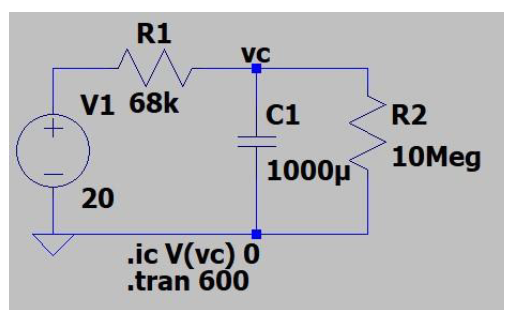
\includegraphics[width=\linewidth]{Figura1.png}
    \caption{Circuito per la carica del condensatore}
    \label{figura1}
\end{figure}

\subsection{Metodologia di misura}
\subsubsection{Carica del condensatore}
Dopo aver costruito il circuito in Figura 1, per il processo di carica del condensatore si è stata inserita la label \emph{vc} su una estremità del condensatore. In seguito, sono state fornite due direttive in Spice: la prima\emph{.ic V(vc) 0} affinché la differenza di potenziale tra il nodo segnato con \emph{vc} e il riferimento (segnato dal triangolo in basso a sinistra della Figura 1) fosse nulla all’istante iniziale; la seconda \emph{.tran 600} per far si che il periodo di simulazione del circuito fosse di 600 secondi, come indicato nella direttiva. Successivamente, si è avviata la simulazione e, utilizzando le sonde predefinite da \emph{LTSpice} ai capi del condensatore, si è acquisito il grafico di $V_C$ e successivamente ottenuti i valori numerici di tensione e relativo istante di tempo.
\subsubsection{Scarica del condensatore}
Per l'analisi del processo di scarica del condensatore, lo sperimentatore ha simulato un circuito con stessa resistenza $R_1$, medesima capacità fornita dal catalogo e stessa resistenza $R_2$, posta in parallelo alla capacità, rappresentante il voltmetro digitale, ma senza generatore, facendo attenzione a mantenersi nelle medesime condizioni iniziali del caso precedente. Inoltre, con la direttiva \emph{.ic V(vc) 20} si è potuta considerare la differenza di potenziale tra il nodo indicato con l’etichetta \emph{vc} e \emph{ground}, inizialmente pari a 20V (esattamente quelli ottenibili dalla carica completa del condensatore precedentemente analizzata). Il circuito così descritto è rappresentato in figura 2.
\begin{figure}
    \centering
    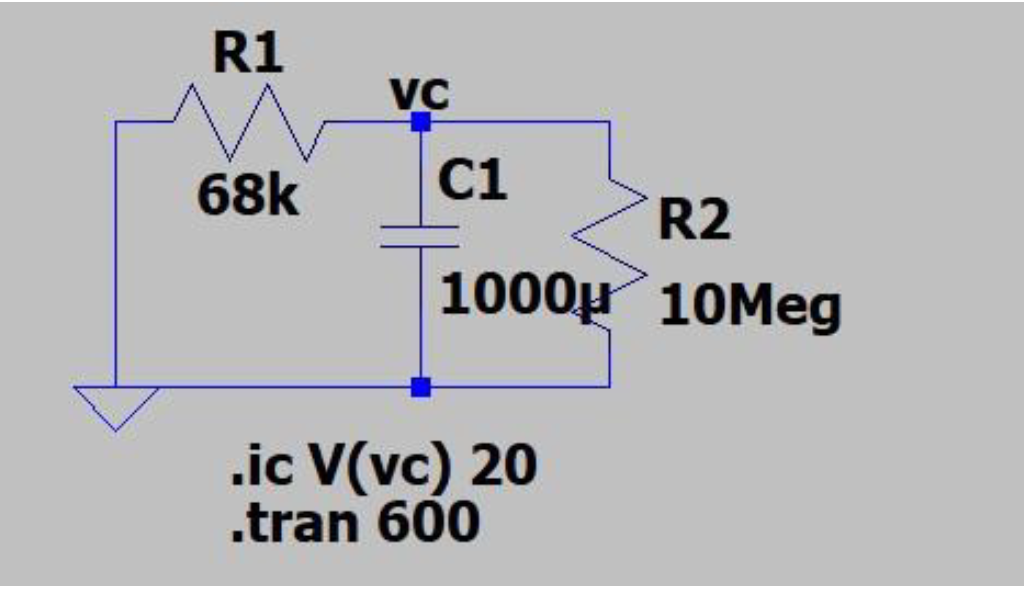
\includegraphics[width=\linewidth]{Figura2.png}
    \caption{Circuito per la fase di scarica}
    \label{figura2}
\end{figure}
È necessario fare una precisazione:  dal momento che il tempo necessario per la carica completa del condensatore è infinito, in un esperimento reale al momento dell’estromissione del generatore la tensione ai capi del condensatore non è esattamente di 20V, come ipotizzato nel secondo circuito della nostra simulazione. Come precedentemente annunciato, dopo 10 minuti, la differenza sebbene non nulla risulta essere trascurabile anche per le tensioni.
I medesimi passaggi sono stati effettuati per lo studio della scarica del condensatore, avviando la simulazione e ottenendo il grafico di $V_C$ in funzione del tempo con i rispettivi valori per relativo istante di tempo.

\section{Analisi dei dati e presentazione dei risultati}
\subsection{Analisi dei dati}
L'analisi dei dati ottenuti dalle varie simulazioni è stata fatta su \emph{Excel}, su cui si sono tabulati i valori di tempo, tensione ai capi del condensatore e resistore. Per il calcolo della costante di tempo dei circuiti è stato necessario calcolare il logaritmo naturale della tensione ai capi della resistenza nel circuito di carica; invece, nel caso del processo di scarica sono stati effettuati gli stessi passaggi per la tensione ai capi del condensatore. Il motivo di questa scelta risiede nel poter considerare le due relazioni lineari; la prima per il processo di carica:
\begin{equation}
    V_R = \varepsilon e^{-\frac{t}{RC}}
\end{equation}
la quale diventa
\begin{equation}
    \ln(V_R) = \ln( \varepsilon ) - \frac{t}{RC}
\end{equation}
mentre per il processo di scarica:
\begin{equation}
    V_C = \varepsilon e^{-\frac{t}{RC}}
\end{equation}
esso diventa
\begin{equation}
    \ln(V_C) = \ln( \varepsilon ) - \frac{t}{RC}
\end{equation}
Risulta evidente che, riportando in un grafico $\ln V_R$ e $\ln V_C$ rispetto al tempo, si ottengono due grafici lineari, la cui pendenza è $ m = −\frac{1}{RC}$, da cui si può facilmente ricavare che $C = - \frac{1}{mR}$, con m coefficiente angolare appena ricavato.

\subsubsection{Errori e incertezze di misura per la simulazione}
Dal momento che l'esperienza è stata effettuata mediante una simulazione, essa è priva di incertezze sperimentali. Tuttavia, risulta logico che in un’esperienza reale errori di natura statistica e sistematica inficerebbero qualsiasi misurazione e dato ottenuto. In particolare, per effettuare la misura e ricreare tale esperienza è utile usare un voltmetro digitale ed un cronometro. Per il cronometro si può valutare come incertezza quella legata alla risoluzione dello strumento, ossia metà della tacca fondamentale della sua scala graduata nel caso sia analogico o metà dell’ultima cifra decimale nel caso sia digitale. Diversa è la situazione per il voltmetro digitale: trattandosi di uno strumento di misura di una grandezza elettrica (nello specifico un multimetro digitale con display a $3\frac{1}{2}$ digit), si valuta l’incertezza associata ad ogni misura con la seguente formula:
\begin{equation}
    u_V = \frac{1}{\sqrt{3}}(0.5\% lettura + 1Digit)
\end{equation}
Per il calcolo dell’incertezza delle grandezze correlate si usa la formula di propagazione dell’errore; in particolare, per questa esperienza:
\begin{equation}
    u_{\ln V_R}^2 = \Bigl ( \frac{\partial \ln V_R}{\partial V_R} \Bigl )^2 u_{V_R}^2
\end{equation}
\subsubsection{Carica del condensatore}
Qui di seguito riportiamo i grafici e i dati relativi al processo di carica del condensatore. I dati e la loro rappresentazione sono riferiti ai primi 5 minuti, tempo in cui scorre una quantità non trascurabile di corrente nel ramo del circuito con il condensatore. Infine, è riportata la tabella con i dati dei restanti 5 minuti e i relativi grafici, realizzati considerando tutti i valori.\footnote{Si noti che tale grafico è stato prodotto con il programma di elabolazione di dati \emph{Excel} a scopo dimostrativo, mentre il grafico da cui ricaviamo la pendenza è stato realizzato con \emph{Root}} \\ Nel grafico in scala non logaritmica non ci sono variazioni significative rispetto al modello teorico. Invece, nel grafico in scala logaritmica vi è una divergenza dal comportamento lineare per tempi molto grandi,dovuta al fatto che la resistenza del voltmetro è grande ma non infinita; questo permette a un piccolo quantitativo di corrente di scorrere nel circuito proprio attraverso il voltmetro. Si faccia riferimento alle figure 3, 4, 5, 6, 7.
\subsubsection{Scarica del condensatore}
Nella seguente sezione si riportano i grafici e i dati relativi al processo di scarica del condensatore.
\subsection{Risultati}
Dall’elaborazione del processo di carica si ottiene un valore di capacità pari a 1.089 ± 0.034mF; invece, dal processo di scarica si ottiene 0.993 ± 0.000(229)mF.\footnote{L’errore è irrilevante poiché si tratta di una simulazione; il suo utilizzo è limitato al calcolo della media ponderata.}
Effettuando la media ponderata otteniamo il valore di 0.993 ± 0.000(229)mF.\footnote{L’incertezza è irrilevante, dato che si è presa in considerazione una simulazione; si è calcolata unicamente per scopi didattici.}

\begin{figure}
    \centering
    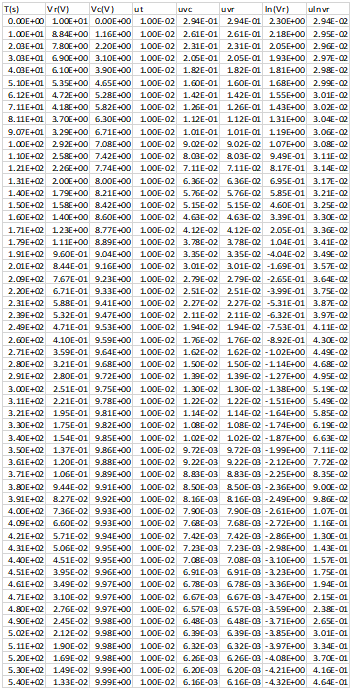
\includegraphics{rel2-tabella_carica.png}
    \caption{Tabella dei valori dei tempi, tensione ai capi di C, tensione ai capi di R e logaritmo naturale di quest’ultimo, relativi al processo di carica.}
    \label{figura3}
\end{figure}

\begin{figure}
    \centering
    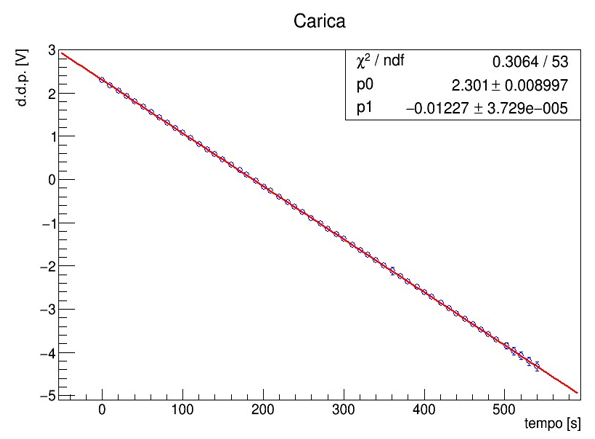
\includegraphics[width=\linewidth]{rel2-grafico_carica.png}
    \caption{Grafico semilogaritmico della tensione ai capi di R e tempi con fit lineare e coefficienti relativi riferito al processo di carica.}
    \label{figura4}
\end{figure}

\begin{figure}
    \centering
    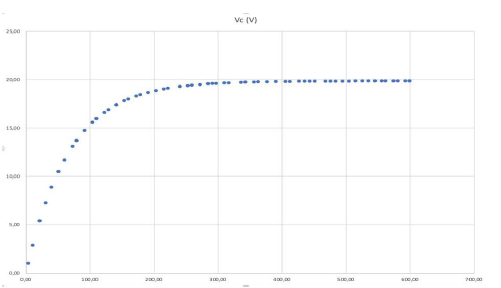
\includegraphics[width=\linewidth]{Figura5.png}
    \caption{Grafico della tensione ai capi di C e tempi nell’intervallo di 10 minuti, relativo al processo di carica.}
    \label{figura5}
\end{figure}

\begin{figure}
    \centering
    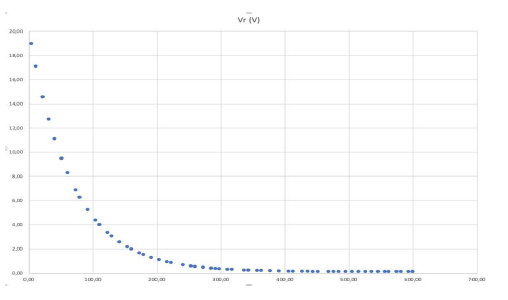
\includegraphics[width=\linewidth]{Figura6.png}
    \caption{Grafico della tensione ai capi di R e tempi nell’intervallo di 10 minuti, relativo al processo di carica.}
    \label{figura6}
\end{figure}

\begin{figure}
    \centering
    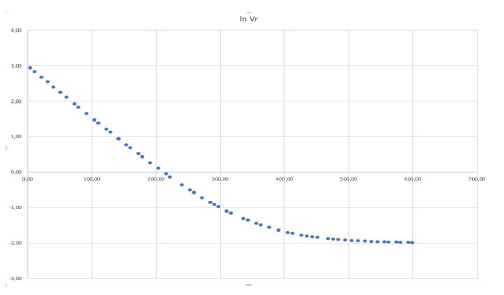
\includegraphics[width=\linewidth]{Figura7.png}
    \caption{Grafico semilogaritmico della tensione ai capi di R e tempi nell’intervallo di 10 minuti, relativo al processo di carica.}
    \label{figura7}
\end{figure}

\begin{figure}
    \centering
    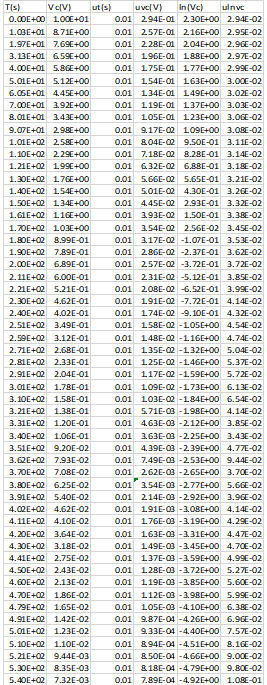
\includegraphics{rel2-tabella_scarica.png}
    \caption{Tabella dei dati di tempo, tensione ai capi del condensatore C e logaritmo di quest’ultima, durante il processo di scarica.}
    \label{figura8}
\end{figure}

\begin{figure}
    \centering
    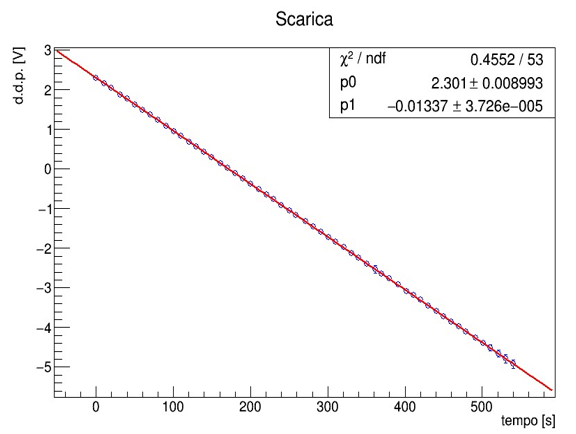
\includegraphics[width=\linewidth]{rel2-grafico_scarica.png}
    \caption{Grafico semilogaritmico di tensione ai capi del condensatore C e tempi con fit lineare e coefficienti relativi, durante il processo di scarica.}
    \label{figura9}
\end{figure}

\end{document}